\chapter{Stochastic RL-MPC}
\label{chapter:stochastic_RL_MPC}

This chapter outlines the performance gains of various RL-MPC implementations as selected from \autoref{chapter:deterministic_RL_MPC} in a stochastic environment. The initial performances of the standalone RL agents and MPC in various levels of uncertainty will be investigated followed by comparisons with the RL-MPC implementations. This chapter seeks to demonstrate the effectiveness of RL-MPC controllers in a realistic setting, providing insight into the controller's potential performance in real-world applications.

\section{Initial RL and MPC Performance}
The uncertainty present in the environment, as mentioned in \autoref{section:experimental-setup}, is characterised as parametric uncertainty. This uncertainty affects the parameters utilised in the computation of the system's outputs (output noise). Consequently, it is customary to use a state estimator for MPC to mitigate this noise. An approach that is both common and effective for MPC is to use the Moving Horizon Estimation (MHE) technique, which can be naturally integrated into the MPC framework. However, this thesis does not incorporate such an estimator in order to clearly observe the impact of combining RL with MPC in a stochastic environment. Moreover, RL was trained on a stochastic environment and the learned policy inherently takes the uncertainty into account. Finally, it is also important to note that for each level of uncertainty a new agent was trained (see \autoref{section:rl-stochastic-results}). Unless specified otherwise, it can be assumed that the corresponding agent is used for each uncertainty level, both in the RL and RL-MPC controllers. Performance metrics include the mean and variance of the final cumulative reward achieved (averaged across 30 simulations). The computational time required to calculate a control action is not considered, as the presence of uncertainty does not affect it.


\begin{figure}[H]
	\centering
	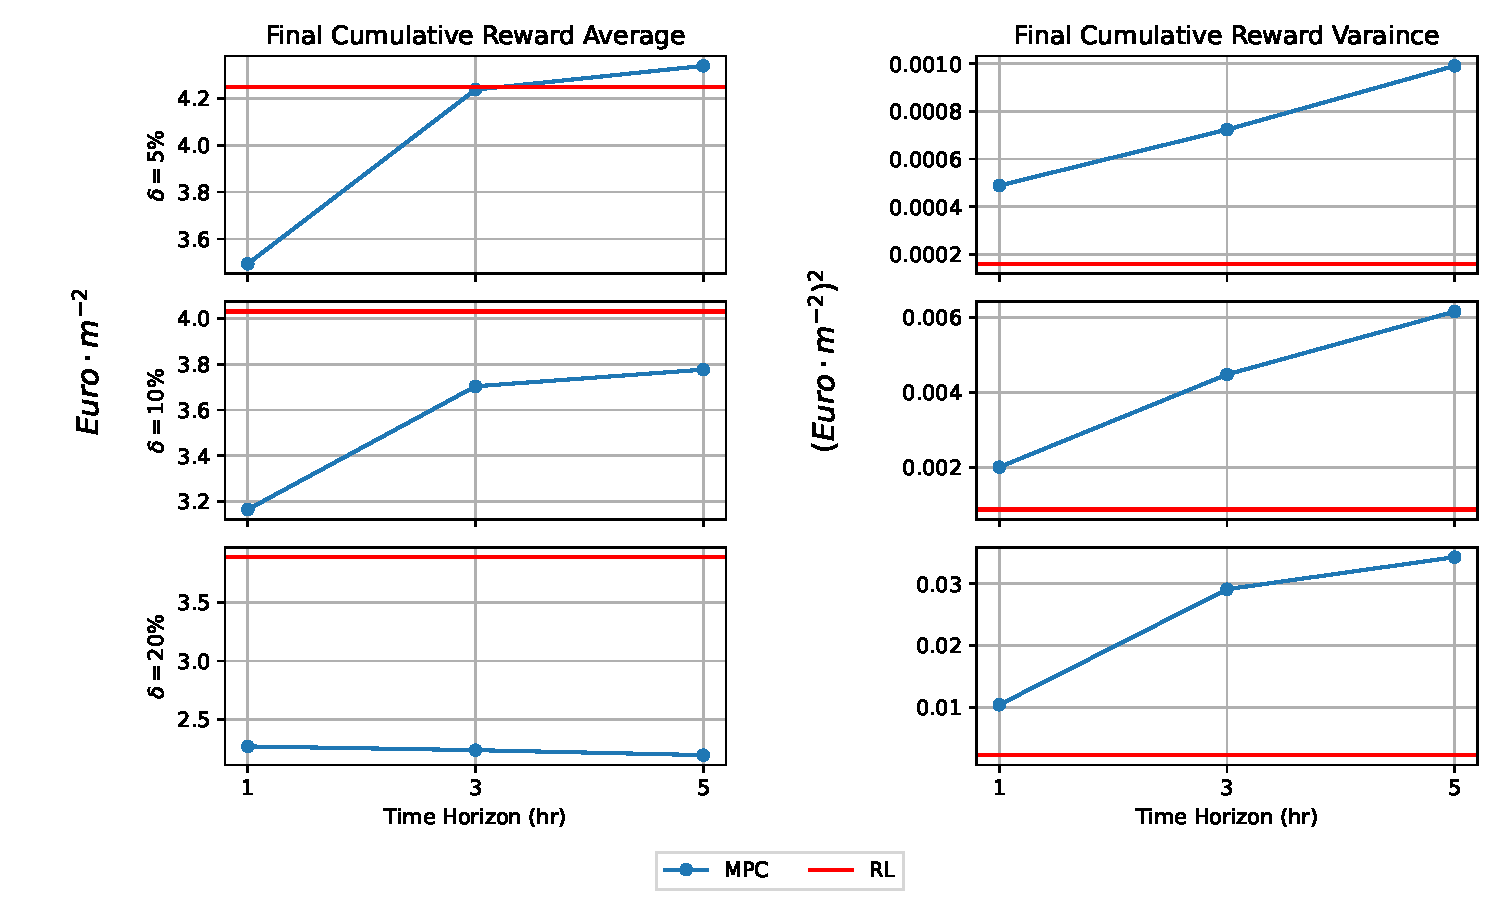
\includegraphics[width=\textwidth]{figures/stochastic_rl_vs_mpc.pdf}
	\caption{RL vs MPC in stochastic conditions}
	\label{fig:stochastic-rl-vs-mpc}
\end{figure}

\autoref{fig:stochastic-rl-vs-mpc} demonstrates the performance of RL and MPC for each prediction horizon and uncertainty level. Contrary to the nominal case shown in \ref{fig:rl-vs-mpc-nominal}, RL consistently outperforms MPC for all prediction horizons and demonstrates superior performance particularly when faced with higher levels of uncertainty. The variance obtained through RL is significantly lower than that of MPC, indicating even greater performance superiority. While it is not surprising given that RL was trained on stochastic data, the findings from \autoref{fig:stochastic-rl-vs-mpc} indicate that as uncertainty levels increase, the effect of increasing the prediction horizon on performance improvement diminishes and may even hinder the performance of MPC in extreme cases of uncertainty. Furthermore, it is worth noting that while both MPC and RL demonstrate comparable performance under conditions of low uncertainty, the final cumulative reward of MPC exhibits significantly higher variance compared to RL. This highlights the robustness of the RL policy. It is investigated whether this robustness to uncertainty is also applied to the RL-MPC controllers.\\
As stated in \autoref{section:final-rl-mpc-nominal}, RL-MPC 3 (which includes a terminal region constraint) and RL-MPC 5 (which includes both a terminal region constraint and a value function as a terminal cost function) are evaluated at different levels of uncertainty. The performance of these implementations is then compared to that of the standalone RL and MPC controllers. The reference trajectory is generated by the RL agent and is based on deterministic predictions.





\section{Results - VF and Terminal Region}


\begin{figure}[H]
	\centering
	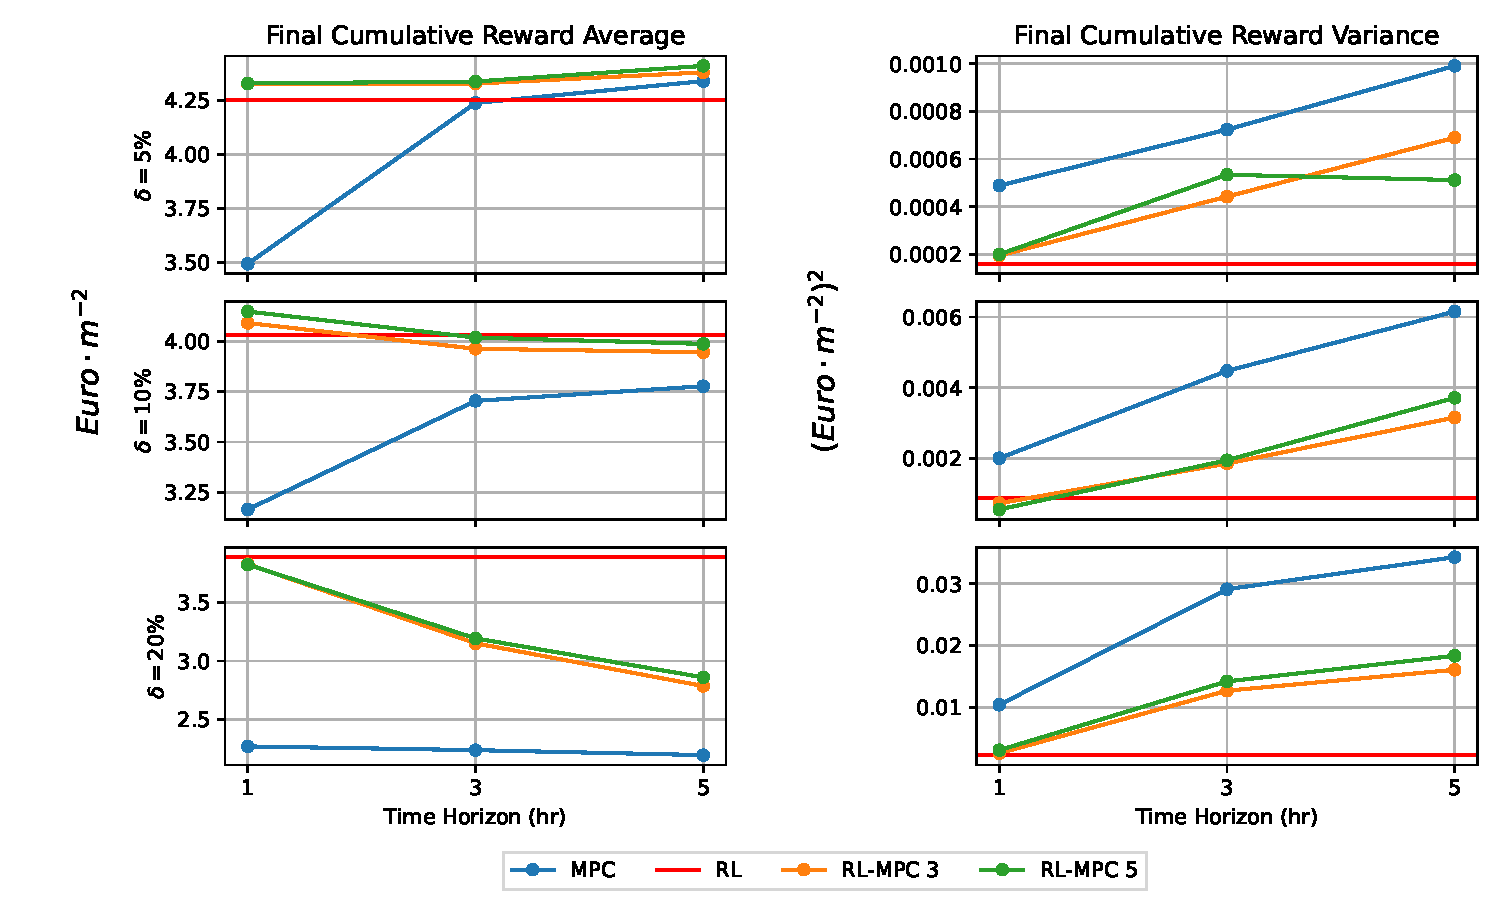
\includegraphics[width=\textwidth]{figures/stochastic_rl_vs_mpc_impl3.pdf}
	\caption{MPC vs stochastic RL vs stochastic RL-MPC 3 and RL-MPC 5}
	\label{fig:stochastic-mpv-vs-rl-rlmpc3-vs-rlmpc5}
\end{figure}

The performance comparison between RL-MPC 3 and RL-MPC 5 in a stochastic environment, as well as their comparison with standalone RL and MPC controllers, is shown in \autoref{fig:stochastic-mpv-vs-rl-rlmpc3-vs-rlmpc5}. Similarly to the nominal case, it is evident that when uncertainty is low ($\delta = 5\%$), the RL-MPC controllers outperform both RL and MPC in terms of the mean final cumulative reward. However, it appears that the variance of the resulting RL-MPC controllers is notably greater than that of RL controllers, but notably lower than that of MPC controllers. It appears as if the variance is averaged between the two controllers. 
However, the behaviour of the RL-MPC controllers becomes intriguing when faced with higher levels of uncertainty. It seems that when there is a high degree of uncertainty, the performance of the RL-MPC controller is significantly impacted due to the poor performance of MPC in such highly stochastic environments. The same can be seen for the variance. While the performance of RL-MPC in a stochastic environment with a $\delta = 10\%$  is comparable to that of RL, it is evident that increasing the prediction horizon significantly affects performance, since it brings the RL-MPC's performance closer to that of MPC. For an uncertainty level of $\delta = 20\%$ the RL-MPC performance is drastically impacted by an increase in prediction horizon, however it still outperforms MPC. A general trend is that as the prediction horizon increases, the RL-MPC controller becomes more similar to the MPC controller. Conversely, with shorter prediction horizons, it becomes more similar to the RL policy. Due to the performance superiority of RL, for higher levels of uncertainty, it is desirable to keep the RL-MPC prediction horizon as short as possible in order to achieve performance, in terms of both the mean and variance of the final cumulative reward. Furthermore, it is clear that the inclusion of a value function as a terminal cost function, in conjunction with a terminal region, has improved performance when compared to using only a terminal region (RL-MPC 3 vs RL-MPC 5). This behaviour is similar to what is observed in the nominal case.

In practice, the exact uncertainty of a model is not known, thus a conservative estimate of uncertainty is assumed during the development of a controller. A parametric uncertainty of $\delta = 20\%$ may be considered too conservative, and if the model and environment is well known, it could have a detrimental effect on performance to design a controller on such a high level of uncertainty. Similarly for when developing a controller assuming a low parametric uncertainty. Therefore a controller is usually developed assuming a middle ground uncertainty level. Thus, it was determined to examine the effectiveness of the RL-MPC controller when designed with an uncertainty level of $\delta = 10\%$ and evaluated under different uncertainty levels. This evaluation was compared to an RL agent that was also trained with an uncertainty level of $\delta = 10\%$ and the nominal MPC. Moreover, it can be seen in \autoref{fig:stochastic-mpv-vs-rl-rlmpc3-vs-rlmpc5}, that careful consideration must be taken when selecting a predication horizon for both RL-MPC and MPC since a longer prediction horizon may lead to substantially worse performance due to the accumulation of uncertainty across the prediction horizon. Thus, a prediction horizon of 3 hours was chosen for both  MPC and RL-MPC 5 (since this is the best performing RL-MPC controller), which was considered to be a suitable compromise for this study.



\begin{figure}[H]
	\centering
	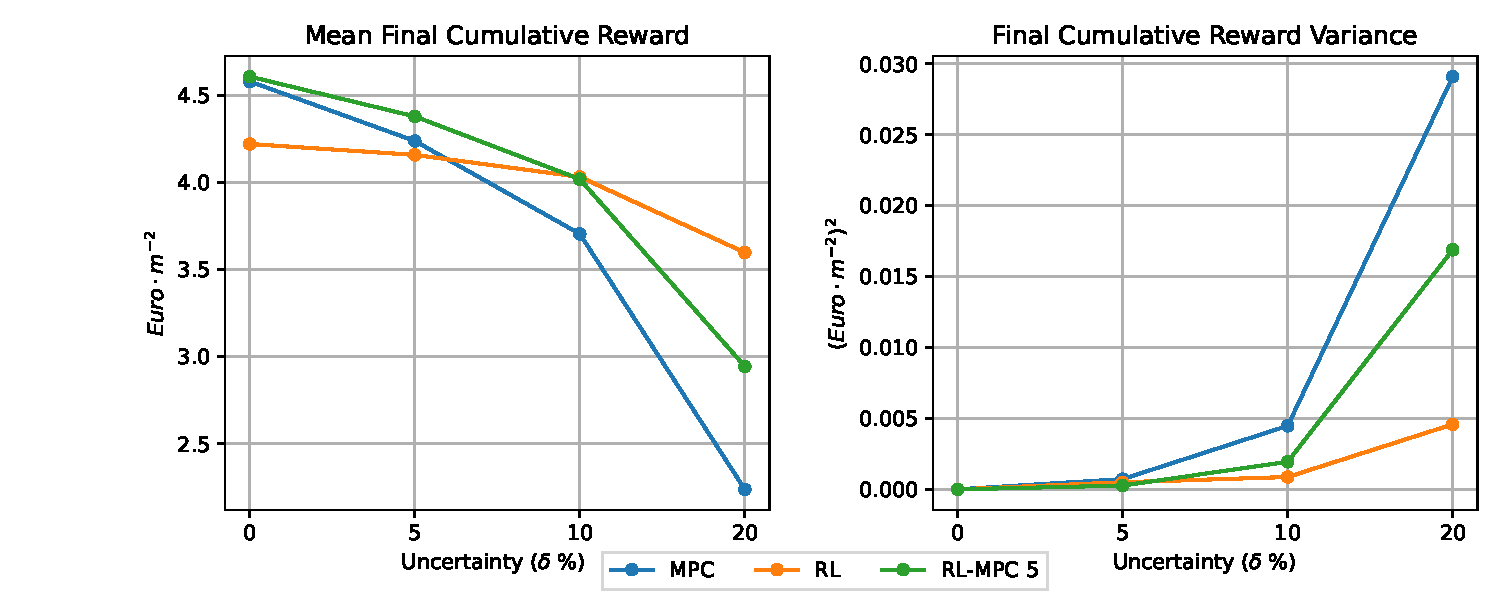
\includegraphics[width=\textwidth]{figures/stochastic_realife.pdf}
	\caption{MPC vs RL vs RL-MPC 5 using an RL agent trained on $\delta = 10\%$ uncertainty and prediction horizon of 3 hours for both MPC and RL-MPC}
	\label{fig:stochastic-reallife}
\end{figure}

The performance of the RL-MPC controller under various levels of parametric uncertainty is shown in \autoref{fig:stochastic-reallife}. Both the the RL-MPC controller and the RL agent are designed on an RL agent trained on a $\delta = 10\%$. The superiority of the RL-MPC controller over both the MPC and RL controllers under normal conditions is once again demonstrated in \autoref{fig:stochastic-reallife} in terms of mean final cumulative reward. This trend persists  until the uncertainty reaches a threshold where the MPC framework is unable to handle it, resulting in a significant decline in performance, which in turn negatively impacts the RL-MPC's performance. Nevertheless, the RL-MPC consistently outperforms the MPC in terms of mean final cumulative reward, and the decrease in performance is not as severe when compared to MPC. The RL-MPC controller also outperforms the MPC controller in terms of variance in the final cumulative reward. However, the RL agent continues to demonstrate superior performance in terms of variance under conditions of increased uncertainty. Nevertheless, is clear that the ability of RL to deal with uncertainty has been partially transferred to the RL-MPC controller. It is mentioned again that no state estimator is employed in the MPC's framework. By implementing this approach, the performance of the MPC is likely to significantly enhance under conditions of high uncertainty. As a result, the performance of the RL-MPC is also expected to improve, and potentially outperforming RL even at high levels of uncertainty. Moreover, if a stochastic MPC was used, such as in \cite{boersmaRobustSamplebasedModel2022}, performance of both MPC and RL-MPC controllers could be even greater. 


\section{Conclusion}

This chapter has demonstrated the performance gains of the RL-MPC controller in a stochastic environment, which builds upon the deterministic evaluations performed in \autoref{chapter:deterministic_RL_MPC}. These results highlights the effectiveness of the RL-MPC controller as well as its robustness in varying levels of uncertainties.\\
The initial experiments conducted a comparison between standalone RL agents (trained on the stochastic data) and an MPC controller. The results consistently showed that RL outperformed MPC in terms of performance across all prediction horizons and uncertainty levels, except for cases with very low uncertainty and a long prediction horizon. Furthermore, RL's capacity to manage uncertainty was further demonstrated by the significantly reduced variance in the final cumulative reward, in comparison to MPC. This level of robustness is essential for practical applications in which uncertainty is a common problem.\\
Further analysis evaluated RL-MPC controllers, specifically RL-MPC 3 and RL-MPC 5, under different uncertainty levels. The findings indicate that RL-MPC controllers consistently outperform the MPC controller and the RL controller when uncertainty is low. However, as uncertainty increases, the performance of RL-MPC approaches that of MPC, especially with longer prediction horizons, resulting in inferior performance as compared to RL. This trend suggests that shorter prediction horizons are preferable for maintaining the superior performance of RL policies within the RL-MPC framework. Moreover, incorporating a value function as a terminal cost function, as in RL-MPC 5, consistently enhances performance over using only a terminal region. Therefore the addition of the value function as a cost function sees benefit in both a deterministic and stochastic setting. 

In real-world scenarios, exact uncertainty levels are often unknown, necessitating conservative estimates during controller development. The performed study with a conservative uncertainty level of $\delta = 10\%$ shows that the  RL-MPC controller, with a prediction horizon of 3hrs, can effectively manage varying uncertainty levels, outperforming both RL and MPC at low uncertainty levels with a more gradual drop in performance at higher uncertainty levels as compared to MPC, indicating that the RL-MPC controller has a higher level of robustness. The MPC framework may be adapted in order to accommodate for uncertainty, specifically a state estimator for output uncertainty and a sample-based approach for model parametric uncertainty  as developed in \cite{boersmaRobustSamplebasedModel2022}. By implementing this approach, the performance and robustness of the MPC can be expected to improve in a stochastic environment. Furthermore, if these methodologies is also applied to the RL-MPC framework, even greater performance and robustness improvements can be anticipated.

In conclusion, this chapter has demonstrated that the RL-MPC controller is a highly efficient controller, even in a stochastic environment. While RL still performs better than the RL-MPC controller under extreme levels of uncertainty, significant performance enhancements can be achieved at low uncertainty levels.
